\documentclass[tikz,border=16pt]{standalone}
\usepackage{tikz}
\usetikzlibrary{arrows.meta,positioning,fit,backgrounds}

% ── Palette ─────────────────────────────────────────────────────────────────
\definecolor{GT}{RGB}{29,78,216}      % blue-700
\definecolor{GTbg}{RGB}{219,234,254}  % blue-100
\definecolor{FD}{RGB}{180,83,9}       % amber-700
\definecolor{FDbg}{RGB}{255,237,213}  % amber-100
\definecolor{PP}{RGB}{71,85,105}      % slate-600
\definecolor{PPbg}{RGB}{241,245,249}  % slate-100
\definecolor{OB}{RGB}{15,23,42}       % near-black

% ── Styles ──────────────────────────────────────────────────────────────────
\tikzset{
  % tall condition label
  gcond/.style={
    draw=GT, fill=GTbg, rounded corners=6pt,
    text width=28mm, minimum height=28mm,
    align=center, inner sep=6pt,
    font=\small\bfseries\sffamily, text=GT
  },
  fcond/.style={
    draw=FD, fill=FDbg, rounded corners=6pt,
    text width=28mm, minimum height=28mm,
    align=center, inner sep=6pt,
    font=\small\bfseries\sffamily, text=FD
  },
  % source data
  gsrc/.style={
    draw=GT, fill=GTbg!45, rounded corners=4pt,
    text width=26mm, minimum height=13mm,
    align=center, inner sep=4pt,
    font=\small\sffamily, text=GT
  },
  fsrc/.style={
    draw=FD, fill=FDbg!45, rounded corners=4pt,
    text width=26mm, minimum height=13mm,
    align=center, inner sep=4pt,
    font=\small\sffamily, text=FD
  },
  % identical pipeline
  pipe/.style={
    draw=PP, fill=PPbg, rounded corners=4pt,
    text width=23mm, minimum height=13mm,
    align=center, inner sep=4pt,
    font=\small\sffamily, text=PP
  },
  % output
  outp/.style={
    draw=OB!60, fill=OB, rounded corners=6pt,
    text width=17mm, minimum height=28mm,
    align=center, inner sep=5pt,
    font=\small\bfseries\sffamily, text=white
  },
}

\begin{document}
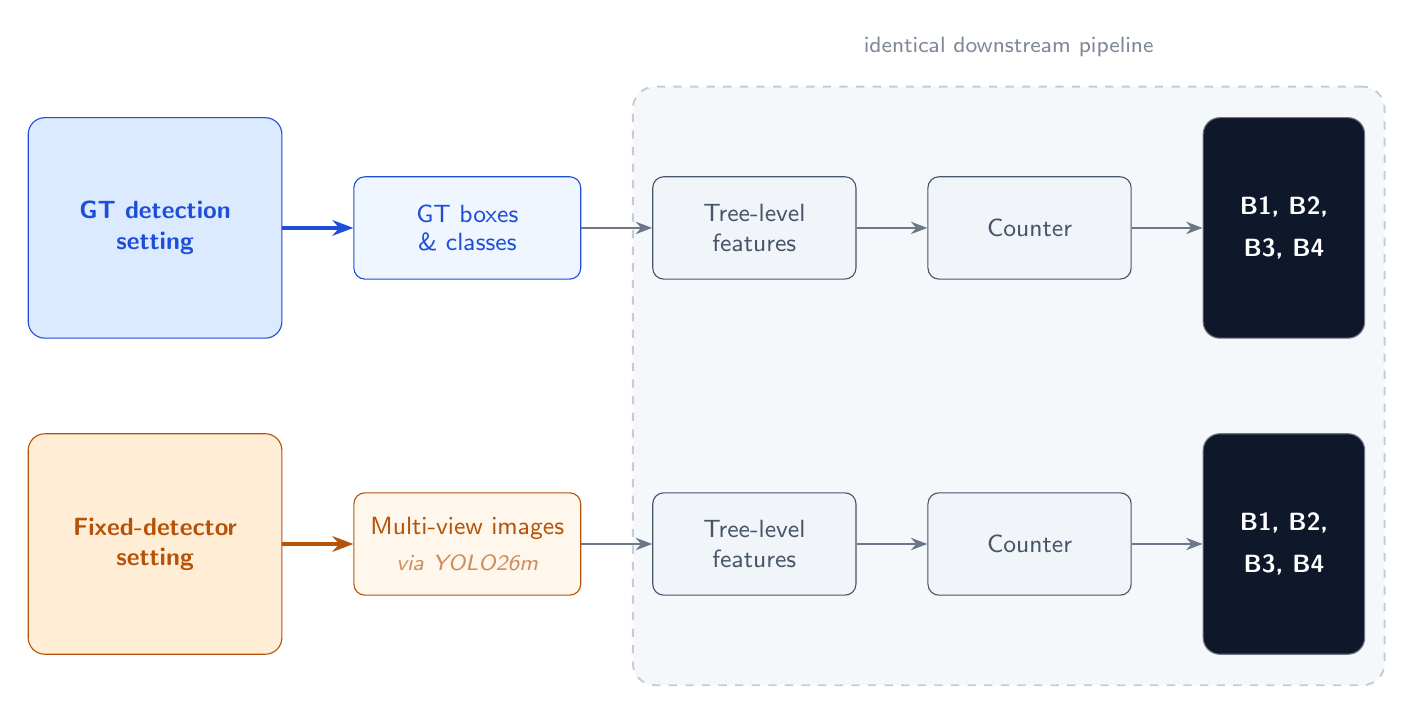
\begin{tikzpicture}[
  font=\small\sffamily,
  node distance=5mm and 9mm,
]

% ── Row 1: GT Detection ──────────────────────────────────────────────────────
\node[gcond] (gtC) {GT detection\\setting};
\node[gsrc, right=of gtC] (gtS) {GT boxes\\[-1pt]\& classes};
\node[pipe, right=of gtS] (gtF) {Tree-level\\features};
\node[pipe, right=of gtF] (gtK) {Counter};
\node[outp, right=of gtK] (gtO) {\textbf{B1, B2,}\\[4pt]\textbf{B3, B4}};

% ── Row 2: Fixed-Detector ───────────────────────────────────────────────────
% Use \mbox to keep "Fixed-detector" unbreakable on one line
\node[fcond, below=12mm of gtC] (fdC)
  {\mbox{Fixed-detector}\\setting};
\node[fsrc, right=of fdC] (fdS) {%
  Multi-view images\\[2pt]%
  {\footnotesize\color{FD!65}\textit{via YOLO26m}}%
};
\node[pipe] (fdF) at (gtF |- fdC) {Tree-level\\features};
\node[pipe] (fdK) at (gtK |- fdC) {Counter};
\node[outp] (fdO) at (gtO |- fdC) {\textbf{B1, B2,}\\[4pt]\textbf{B3, B4}};

% ── Arrows: GT ───────────────────────────────────────────────────────────────
\draw[-{Stealth[scale=0.9]}, very thick, GT]  (gtC) -- (gtS);
\draw[-{Stealth[scale=0.9]}, thick, PP!80]    (gtS) -- (gtF);
\draw[-{Stealth[scale=0.9]}, thick, PP!80]    (gtF) -- (gtK);
\draw[-{Stealth[scale=0.9]}, thick, PP!80]    (gtK) -- (gtO);

% ── Arrows: FD ───────────────────────────────────────────────────────────────
\draw[-{Stealth[scale=0.9]}, very thick, FD]  (fdC) -- (fdS);
\draw[-{Stealth[scale=0.9]}, thick, PP!80]    (fdS) -- (fdF);
\draw[-{Stealth[scale=0.9]}, thick, PP!80]    (fdF) -- (fdK);
\draw[-{Stealth[scale=0.9]}, thick, PP!80]    (fdK) -- (fdO);

% ── Background: identical pipeline section ──────────────────────────────────
\begin{pgfonlayer}{background}
  \node[
    fill=PPbg!70, draw=PP!30, dashed, line width=0.7pt,
    rounded corners=8pt,
    inner xsep=7pt, inner ysep=11pt,
    fit=(gtF)(gtK)(gtO)(fdF)(fdK)(fdO)
  ] (ident) {};
\end{pgfonlayer}

% ── Label ────────────────────────────────────────────────────────────────────
\node[
  above=7pt of ident.north,
  font=\footnotesize\sffamily,
  text=PP!70
] {identical downstream pipeline};

\end{tikzpicture}
\end{document}
